\chapter{Etude Conceptuel}
\section{Présentation de la méthode de conception}
\subsection{Merise}
Merise est une méthode d'analyse, de conception et de gestion de projet
informatique.
Merise a été très utilisée dans les années 1970 et 1980 pour l'informatisation
massive des organisations. Cette méthode reste adaptée pour la gestion des
projets internes aux organisations, se limitant à un domaine précis. Elle est en
revanche moins adaptée aux projets transverses aux organisations, qui gèrent le
plus souvent des informations à caractère sociétal (environnemental et social)
avec des parties prenantes.
Merise procède à un traitement séparé des données et des processus, où la vue
des données est modélisée en trois étapes : de la conception à la physique en
passant par la logique. De même, la vue axée sur les processus passe par les
trois étapes conceptuelle, organisationnelle et opérationnelle. Ces étapes du
processus de modélisation sont parallèles aux étapes du cycle de
vie: planification stratégique, étude préliminaire, étude détaillée,
développement, mise en œuvre et maintenance. C'est une méthode d'analyse
basée sur le modèle entité-relation.
En utilisant Merise, vous pouvez concevoir des tables avec des relations pour
créer une base de données relationnelle.
\subsection{Tableau des models}
\begin{table}[ht]
    \begin{tabularx}{\textwidth}{|X|X|X|}
    
        \hline
        \textbf{Niveau}    & \textbf{Données} & \textbf{Traitements}  \\
        \hline
        conceptuel & Modèle conceptuel de données (MCD) & Modèle conceptuel de traitements (MCT) \\
        \hline
        organisationnel & Modèle logique de données (MLD) & Modèle organisationnel de traitements (MOT)  \\
        \hline
        technique & Modèle physique de données (MPD) & Modèle opérationnel et physique des traitements (MOPT) \\
        \hline
    \end{tabularx}
\end{table}
\subsection{Niveau conceptuel}
A ce niveau le système d'information est représenté indépendamment de
l'organisation et du moyen physique et informatique qu'il pourrait utiliser. Il
repent au « quoi ? » et « que veut-on faire ? ».
Les modèles proposés par merise à ce niveau sont :
\begin{itemize}
    \item Modèle conceptuel de données (MCD)
    \item Modèle conceptuel de traitements (MCT)
\end{itemize}

\subsection{Niveau organisationnel et logique}
A ce niveau  on fait les choix organisationnels ; le système d'information est
représenté en tenant compte des contraintes imposées par ce choix. L'objectif
de ce niveau est rependre aux questions « quelle ? Quand ? Ou ? »
Les modèles proposés par Merise sont :
\begin{itemize}
    \item Modèle logique de données (MLD)
    \item Modèle organisationnel de traitements (MOT)
\end{itemize}

\subsection{Niveau opérationnel et physique}
A ce niveau sont intégrées les moyens techniques au projet ; il s’expriment en
terme de matériels ou logiciels  qui permet de rependre à la question
comment? Avec quel moyen.
Les modèles proposés par merise sont :
\begin{itemize}
    \item Modèle physique de données (MPD)
    \item Modèle opérationnel et physique des traitements (MOPT)
\end{itemize}

\section{Dictionnaire des données}
\subsection{Définition}
Dictionnaire de données est le résultat de l'épuration de données extraites
des documents en éliminant les synonymes, les polysémies, les champs
calculable et non important et en ajoutant les rubriques nécessaires à
l'automatisation.
 On appel synonyme deux informations ayant le même sens mais des
noms déférents.
 On appel polysémies deux informations ayant le même nom mais des
sens déférents.
 Eliminer les données calculables.
 Eclater les données qui contiennent plusieurs informations.
* Pour chaque donnée il faut préciser :
- Sa désignation
- Sa longueur
- Un code
- Son type
\subsection{epuration de Dictionnaire des données}
\begin{itemize}
    \item \textbf{pas de synonymes} \\ \textbf{exemple:} nom et prenom,nom et prenom de demandeur,nom et prenom de stagiare
    \item \textbf{pas de polysémes} \\ \textbf{exemple:} date > date de rendez-vous,date inventaire,\dots, qt > quantite demande,quantite achete 
    \item \textbf{pas de données concatenes} \\\textbf{exemple:} nom et prenom > nom,prenom
    \item \textbf{ilya des données calculable} \\\textbf{exemple:} ecart = qt theorique - qt physique 
    \item \textbf{données unnutiles} \\ pas de données unnutiles
    \item \textbf{données rajoute} \\\textbf{exemple:} code de maintenance,code d'experience 
\end{itemize}
\subsection{Dictionnaire des données épurée}
\csvreader[
  longtable=|l|l|c|c|,
  table head=\caption{Dictionnaire des données\label{tab:sometab}}\\ \hline
    \bfseries desgination &\bfseries code &\bfseries type &\bfseries taill \\ \endfirsthead\hline,
  late after line=\\,table foot=\hline,
]{chapter/Conceptual Study/dd.csv}{1=\desgination,2=\code,3=\type,4=\taill}{\desgination&\code&\type&\taill}
\section{Le Modèle conceptuel des données (MCD)}
\subsection{Définition}
schéma représentant la structure du système d'information, du point de vue des
données, c'est-à-dire les dépendances ou relations entre les différentes données
du système d'information
Le MCD repose sur les notions d'entité et d'association et sur les notions de
relations. Le modèle conceptuel des données s'intéresse à décrire la sémantique
du domaine
L'entité est définie comme un objet de gestion considéré d'intérêt pour
représenter l'activité à modéliser (exemple : entité pays). À son tour, chaque
entité (ou objet) est porteuse d'une ou plusieurs propriétés simples, dites
atomiques (exemples : code, nom, capitale, population, superficie) dont l'une,
unique et discriminante, est désignée comme identifiant (exemple : code).
L'association est un lien sémantique entre entités :
 1 entité reliée à elle-même : la relation est dite réflexive,
 2 entités : la relation est dite binaire (ex : une usine 'est implantée' dans
un pays),
 plus rarement 3 ou plus : ternaire, voire de dimension supérieure. En fait,
hormis le cas d'une date (la table date disparaît) si une relation a 3 points
d'attache ou plus, on peut réécrire la relation en transformant la relation
en table et en transformant les liens en relations.
Une association peut également être porteuse d'une ou plusieurs propriétés.
\subsection{les regles de gestion}
Une règle de gestion est une traduction conceptuelle des objectifs choisis et des contraintes acceptées par l'entreprise,  elle plus particulier au traitement (reglz d'action) ou données (règle de calcul).\\
\textbf{exemple}
\begin{itemize}
    \item Le stagiaire appartient à un seul laboratoire, le laboratoire lui appartient plusieur stagiaires
    \item inventaire contient plusieur article, un seul article peut etre contient dans plusieur inventaire
    \item un seul stagiaire peut bénéficier plusieur article, un seul article elle peut par plusieur stagiaire
    \item Une expérience peut contenir plusieurs échantillons, mais un échantillon est contenu dans une seule expérience
\end{itemize}
\subsection{schéma}
\begin{figure}[hbtp]
    \centering
    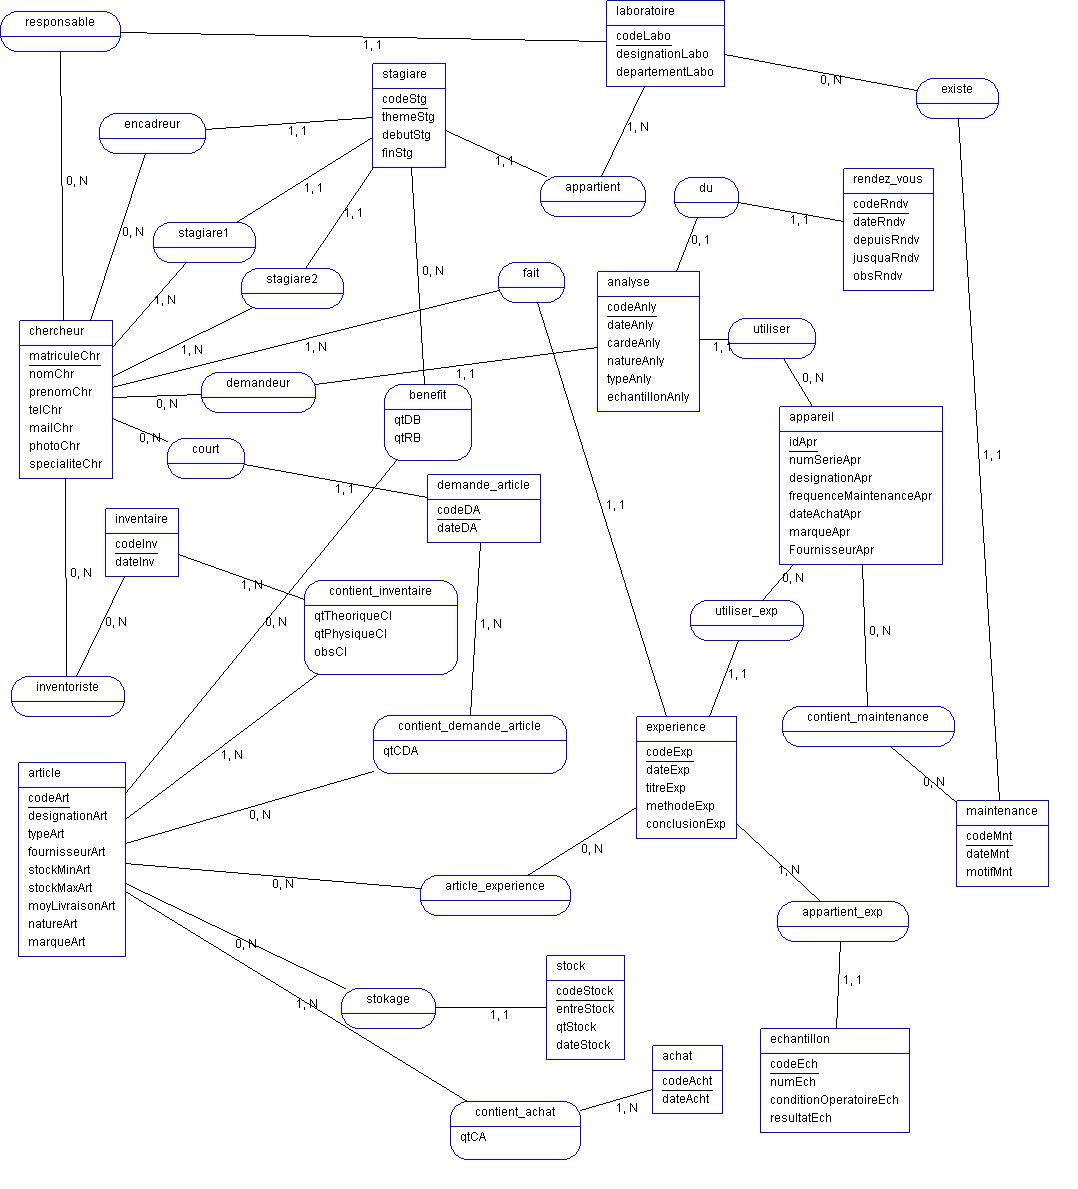
\includegraphics[width=.9\paperwidth]{images/mcd.png}
    \caption{MCD}
    \label{fig:MCD}
  \end{figure}
\newpage
\section{Modèle Logique des Données(MLD)}
\subsection{Définition}
qui reprend le contenu du MCD précédent, mais précise la volumétrie, la
structure et l'organisation des données telles qu'elles pourront être
implémentées. Par exemple, à ce stade, il est possible de connaître la liste
exhaustive des tables qui seront à créer dans une base de données relationnelle
Comme son nom l'indique, l'étude d’organisation s'attache à préciser comment
on organise les données de l'entreprise (MLD) et les tâches ou procédures .
Pour autant, les choix techniques d'implémentation, tant pour les données que
pour les traitements.
\subsection{les ragles de gestion}
\begin{enumerate}
    \item \textbf{Transformation des entités} Toute entité est transformée en table. Les propriétés de l'entité deviennent les
    attributs de la table. L'identifiant de l'entité devient la clé primaire de la table.\\
    \textbf{example:} l entité chercheur devient table, la clé primaire de la table matriculeChr
    \item \textbf{Transformation des relations binaires du type (x,n) – (x,1)} Afin de représenter la relation, on duplique la clé primaire de la table basée sur
    l'entité à cardinalité (x,n) dans la table basée sur l'entité à cardinalité (x,1). Cet attribut
    est appelé clé étrangère.\\
    \textbf{example:} la relation appartient on duplique la clé primaire de la table laboratoire dans la table stagiaire 
    \item \textbf{Relation binaire (0,1)-(1,1)} On duplique la clé de la table basée sur l'entité à cardinalité (0,1) dans la table
    basée sur l'entité à cardinalité (1,1)\\
    \textbf{example:} la relation "DU"  on duplique la clé primaire de la table analyse dans la table rendez\_vous 
    \item \textbf{Transformation des relations binaires du type (x,n) – (x,n)}On crée une table supplémentaire ayant comme clé primaire une clé composée des
    clés primaires des 2 tables. Lorsque la relation contient elle-même des propriétés, celles-ci deviennent attributs de la table supplémentaire. 
    Une propriété de la relation qui estsoulignée devra appartenir à la clé primaire composée de la table supplémentaire\\
    \textbf{example:} la relation contient\_achat  On crée une table supplémentaire contient\_achat. codeAcht,codeArt comme clé primaire composée est des cle étrangère,qtCA  deviennent
    attribut de latable contient\_achat
\end{enumerate}

\subsection{schéma}
\begin{itemize}
    \item \textbf{chercheur} (\underline{matriculeChr}, nomChr, prenomChr, telChr, mailChr, photoChr, specialiteChr)  
    \item \textbf{laboratoire} (\underline{codeLabo}, designationLabo, departementLabo, \#matriculeChr)  
    \item \textbf{article} (\underline{codeArt}, designationArt, typeArt, fournisseurArt, stockMinArt, stockMaxArt, moyLivraisonArt, natureArt, marqueArt)  
    \item \textbf{stock} (\underline{codeStock}, entreStock, qtStock, dateStock, \#codeArt)  
    \item \textbf{appareil} (\underline{idApr}, numSerieApr, designationApr, frequenceMaintenanceApr, dateAchatApr, marqueApr, FournisseurApr)  
    \item \textbf{analyse} (\underline{codeAnly}, dateAnly, cardeAnly, natureAnly, typeAnly, echantillonAnly, \#idApr, \#matriculeChr)  
    \item \textbf{rendez\_vous} (\underline{codeRndv}, dateRndv, depuisRndv, jusquaRndv, obsRndv, \#codeanly)  
    \item \textbf{experience} (\underline{codeExp}, dateExp, titreExp, methodeExp, conclusionExp, \#idApr,\#matriculeChr)  
    \item \textbf{stagiare} (\underline{codeStg}, themeStg, debutStg, finStg, \#encadreur,\#matriculeChr1,\#matriculeChr2 , \#codeLabo)  
    \item \textbf{demande\_article} (\underline{codeDA}, dateDA, \#matriculeChr)  
    \item \textbf{inventaire} (\underline{codeInv}, dateInv)  
    \item \textbf{maintenance} (\underline{codeMnt}, dateMnt, motifMnt, \#codeLabo)  
    \item \textbf{echantillon} (\underline{codeEch}, numEch, conditionOperatoireEch, resultatEch, \#codeExp)  
    \item \textbf{achat} (\underline{codeAcht}, dateAcht)  
    \item \textbf{benefit} (\underline{\#codeArt,\# matriculeChr}, qtDB, qtRB)  
    \item \textbf{contient\_maintenance} (\underline{\#idApr, \#codeMnt})  
    \item \textbf{contient\_demande\_article} (\underline{\#codeDA, \#codeArt}, qtCDA)  
    \item \textbf{inventoriste} (\underline{\#matriculeChr, \#codeInv})  
    \item \textbf{contient\_inventaire} (\underline{\#codeArt, \#codeInv}, qtTheoriqueCI, qtPhysiqueCI, obsCI)  
    \item \textbf{article\_experience} (\underline{\#codeExp, \#codeArt})  
    \item \textbf{contient\_achat} (\underline{\#codeArt, \#codeAcht}, qtCA) 

\end{itemize}
\section{Le modèle physique des données}
est la traduction du modèle logique des données (MLD) dans une structure de
données spécifique au système de gestion de bases de données (SGBD) utilisé.
Passage du MLD au MPD
Le passage MLD à MPD se fait par les étapes suivantes:
Implémentation physique de chaque table du MLD dans le SGBD utilisé.
Pour chaque table, indiquer au SGBD quel(s) champ(s) constitue(nt) la clé
primaire.
Pour chaque table, indiquer au SGBD la (les) clé(s) étrangère(s), et la (les)
clé(s) primaire(s) correspondante(s).


\vspace{2cm}
\begin{tabular}{ |p{5cm}||p{4cm}|p{3cm}|p{3cm}|  }
    \hline
    \multicolumn{4}{|c|}{Nom de la Table: chercheur} \\
    \hline
    \multicolumn{4}{|c|}{Cle primaire : matriculeChr} \\
    \hline
    \multicolumn{4}{|c|}{Cle secondaire : / } \\
    \hline
    \hline
    desgination&code&type&taill \\
    \hline
    prenom de chercheur&prenomChr&AN&50 \\
    mail de chercheur&mailChr&AN&150 \\
    telephone de chercheur&telChr&AN&10 \\
    matricule de chercheur&matriculeChr&AN&13 \\
    photo de chercheur&photoChr&AN&100 \\
    specialite de chercheur&specialiteChr&AN&100 \\
    nom de chercheur&nomChr&AN&50 \\
    \hline
    \hline
    \multicolumn{3}{|c|}{Taille d’enregistrement} & 473\\
    \hline
\end{tabular}

\vspace{2cm}

\begin{tabular}{ |p{5cm}||p{4cm}|p{3cm}|p{3cm}|  }
    \hline
    \multicolumn{4}{|c|}{Nom de la Table: laboratoire} \\
    \hline
    \multicolumn{4}{|c|}{Cle primaire : codeLabo} \\
    \hline
    \multicolumn{4}{|c|}{Cle secondaire : matriculeChr } \\
    \hline
    \hline
    desgination&code&type&taill \\
    \hline
    designation de laboratoire&designationLabo&AN&50 \\
    code de laboratoire&codeLabo&AN&6 \\
    departement&departementLabo&AN&50 \\
    matricule de chef de laboratoire&matriculeChr&AN&13 \\
    \hline
    \hline
    \multicolumn{3}{|c|}{Taille d’enregistrement} & 119\\
    \hline
\end{tabular}

\vspace{2cm}

\begin{tabular}{ |p{5cm}||p{4cm}|p{3cm}|p{3cm}|  }
    \hline
    \multicolumn{4}{|c|}{Nom de la Table: article} \\
    \hline
    \multicolumn{4}{|c|}{Cle primaire : codeArt} \\
    \hline
    \multicolumn{4}{|c|}{Cle secondaire : / } \\
    \hline
    \hline
    desgination&code&type&taill \\
    \hline
    code Produit ou verrerie&codeArt&AN&10 \\
    designation Produit ou verrerie&designationArt&AN&150 \\
    stock minimum de Produit ou verrerie&stockMinArt&N&10 \\
    stock Maximum de Produit ou verrerie&stockMaxArt&N&10 \\
    fournisseur de Produit ou verrerie&fournisseurArt&AN&100 \\
    moyen de Livraison de Produit ou verrerie&moyLivraisonArt&N&3 \\
    type Produit ou verrerie&typeArt&B&1 \\
    nature de Produit ou verrerie&natureArt&AN&50 \\
    marque de Produit ou verrerie&marqueArt&AN&50 \\
    \hline
    \hline
    \multicolumn{3}{|c|}{Taille d’enregistrement} & 384\\
    \hline
\end{tabular}

\vspace{2cm}

\begin{tabular}{ |p{5cm}||p{4cm}|p{3cm}|p{3cm}|  }
    \hline
    \multicolumn{4}{|c|}{Nom de la Table: stock} \\
    \hline
    \multicolumn{4}{|c|}{Cle primaire : codeStock} \\
    \hline
    \multicolumn{4}{|c|}{Cle secondaire :  codeArt} \\
    \hline
    \hline
    desgination&code&type&taill \\
    \hline
    entre ou sorte de stock&entreStock&B&1 \\
    quantite de mouvement de stock&qtStock&N&10 \\
    code de mouvement de stock&codeStock&N&5 \\
    date de mouvement de stock&dateStock&DT&19 \\
    code Produit ou verrerie&codeArt&AN&10 \\
    \hline
    \hline
    \multicolumn{3}{|c|}{Taille d’enregistrement} & 35\\
    \hline
\end{tabular}

\vspace{2cm}

\begin{tabular}{ |p{5cm}||p{4cm}|p{3cm}|p{3cm}|  }
    \hline
    \multicolumn{4}{|c|}{Nom de la Table: appareil } \\
    \hline
    \multicolumn{4}{|c|}{Cle primaire : idApr} \\
    \hline
    \multicolumn{4}{|c|}{Cle secondaire : / } \\
    \hline
    \hline
    desgination&code&type&taill \\
    \hline
    designation d'appareil&designationApr&AN&100 \\
    frequence de Maintenance de l'appreil&frequenceMaintenanceApr&N&2 \\
    date d'achat de l'appareil&dateAchatApr&D&10 \\
    id appareil&idApr&AN&30 \\
    numero serie de l'appareil&numSerieApr&AN&20 \\
    marque  de l'appareil&marqueApr&AN&50 \\
    Fournisseur  de l'appareil&FournisseurApr&AN&100 \\
    \hline
    \hline
    \multicolumn{3}{|c|}{Taille d’enregistrement} & 312\\
    \hline
\end{tabular}

\vspace{2cm}

\begin{tabular}{ |p{5cm}||p{4cm}|p{3cm}|p{3cm}|  }
    \hline
    \multicolumn{4}{|c|}{Nom de la Table: analyse} \\
    \hline
    \multicolumn{4}{|c|}{Cle primaire :codeAnly } \\
    \hline
    \multicolumn{4}{|c|}{Cle secondaire :idApr, matriculeChr  } \\
    \hline
    \hline
    desgination&code&type&taill \\
    \hline
    code d'analyse&codeAnly&N&6 \\
    carde d'analyse&cardeAnly&AN&100 \\
    nature d'analyse&natureAnly&AN&50 \\
    type d'analyse&typeAnly&AN&50 \\
    nombre d'echantillon d'analyse&echantillonAnly&N&2 \\
    date d'analyse&dateAnly&D&10\\
    id appareil&idApr&AN&30 \\
    matricule de chercheur&matriculeChr&AN&13 \\
    \hline
    \hline
    \multicolumn{3}{|c|}{Taille d’enregistrement} & 261\\
    \hline
\end{tabular}

\vspace{2cm}

\begin{tabular}{ |p{5cm}||p{4cm}|p{3cm}|p{3cm}|  }
    \hline
    \multicolumn{4}{|c|}{Nom de la Table:rendez\_vous } \\
    \hline
    \multicolumn{4}{|c|}{Cle primaire : codeRndv} \\
    \hline
    \multicolumn{4}{|c|}{Cle secondaire : codeanly } \\
    \hline
    \hline
    desgination&code&type&taill \\
    \hline
    code de rendez-vous&codeRndv&N&5 \\
    date de rendez-vous&dateRndv&D&10 \\
    depuis&depuisRndv&T&9 \\
    jusqua&jusquaRndv&T&9 \\
    observation de rendez-vous&obsRndv&AN&2000 \\
    code d'analyse&codeAnly&N&6 \\
    \hline
    \hline
    \multicolumn{3}{|c|}{Taille d’enregistrement} & 119\\
    \hline
\end{tabular}

\vspace{2cm}

\begin{tabular}{ |p{5cm}||p{4cm}|p{3cm}|p{3cm}|  }
    \hline
    \multicolumn{4}{|c|}{Nom de la Table: experience} \\
    \hline
    \multicolumn{4}{|c|}{Cle primaire : codeExp} \\
    \hline
    \multicolumn{4}{|c|}{Cle secondaire : idApr,matriculeChr } \\
    \hline
    \hline
    desgination&code&type&taill \\
    \hline
    
    methode d'experience&methodeExp&AN&5000 \\
    titre d'experience&titreExp&AN&150 \\
    code d'experience&codeExp&N&5 \\
    date d'experience&dateExp&D&10 \\
    conclusion d'experience&conclusionExp&AN&5000 \\
    id appareil&idApr&AN&30 \\
    code chercheur&matriculeChr&AN&13 \\
    \hline
    \hline
    \multicolumn{3}{|c|}{Taille d’enregistrement} & 1208\\
    \hline
\end{tabular}

\vspace{2cm}

\begin{tabular}{ |p{5cm}||p{4cm}|p{3cm}|p{3cm}|  }
    \hline
    \multicolumn{4}{|c|}{Nom de la Table:stagiare } \\
    \hline
    \multicolumn{4}{|c|}{Cle primaire : codeStg} \\
    \hline
    \multicolumn{4}{|c|}{Cle secondaire :  encadreur,matriculeChr1,matriculeChr2 , codeLabo} \\
    \hline
    \hline
    desgination&code&type&taill \\
    \hline
    debut de stage&debutStg&D&10 \\
    fin de stage&finStg&D&10 \\
    code stagiares&codeStg&N&5 \\
    theme stage&themeStg&AN&150 \\
    code de laboratoire&codeLabo&AN&6 \\
    matricule de encadreur&encadreur&AN&13 \\
    matricule de chercheur 1&matriculeChr1&AN&13 \\
    matricule de chercheur 2&matriculeChr2&AN&13 \\
    \hline
    \hline
    \multicolumn{3}{|c|}{Taille d’enregistrement} & 220\\
    \hline
\end{tabular}

\vspace{2cm}

\begin{tabular}{ |p{5cm}||p{4cm}|p{3cm}|p{3cm}|  }
    \hline
    \multicolumn{4}{|c|}{Nom de la Table:demande\_article } \\
    \hline
    \multicolumn{4}{|c|}{Cle primaire :codeDA } \\
    \hline
    \multicolumn{4}{|c|}{Cle secondaire :matriculeChr  } \\
    \hline
    \hline
    desgination&code&type&taill \\
    \hline
    code de demande d'article&codeDA&N&5 \\
    date de demande d'article&dateDA&D&10 \\
    matricule de chercheur&matriculeChr&AN&13 \\
    \hline
    \hline
    \multicolumn{3}{|c|}{Taille d’enregistrement} & 28\\
    \hline
\end{tabular}

\vspace{2cm}

\begin{tabular}{ |p{5cm}||p{4cm}|p{3cm}|p{3cm}|  }
    \hline
    \multicolumn{4}{|c|}{Nom de la Table:inventaire } \\
    \hline
    \multicolumn{4}{|c|}{Cle primaire :codeInv } \\
    \hline
    \multicolumn{4}{|c|}{Cle secondaire : / } \\
    \hline
    \hline
    desgination&code&type&taill \\
    \hline
    code inventaire&codeInv&AN&8 \\
    date inventaire&dateInv&D&10 \\
    \hline
    \hline
    \multicolumn{3}{|c|}{Taille d’enregistrement} & 18\\
    \hline
\end{tabular}

\vspace{2cm}

\begin{tabular}{ |p{5cm}||p{4cm}|p{3cm}|p{3cm}|  }
    \hline
    \multicolumn{4}{|c|}{Nom de la Table:maintenance } \\
    \hline
    \multicolumn{4}{|c|}{Cle primaire :codeMnt } \\
    \hline
    \multicolumn{4}{|c|}{Cle secondaire : codeLabo } \\
    \hline
    \hline
    desgination&code&type&taill \\
    \hline
    motif de maintenance&motifMnt&AN&2000 \\
    code de maintenance&codeMnt&AN&10 \\
    date de maintenance&dateMnt&D&10 \\
    code de laboratoire&codeLabo&AN&6 \\
    \hline
    \hline
    \multicolumn{3}{|c|}{Taille d’enregistrement} & 2026\\
    \hline
\end{tabular}

\vspace{2cm}

\begin{tabular}{ |p{5cm}||p{4cm}|p{3cm}|p{3cm}|  }
    \hline
    \multicolumn{4}{|c|}{Nom de la Table: echantillon } \\
    \hline
    \multicolumn{4}{|c|}{Cle primaire : codeEch } \\
    \hline
    \multicolumn{4}{|c|}{Cle secondaire : codeExp } \\
    \hline
    \hline
    desgination&code&type&taill \\
    \hline
    condition operatoire echantillon&conditionOperatoireEch&AN&1000 \\
    resultat de echantillon&resultatEch&AN&1000 \\
    numero d'echantillon&numEch&N&3 \\
    code d'echantillon&codeEch&N&7 \\
    code d'experience&codeExp&N&5 \\
    \hline
    \hline
    \multicolumn{3}{|c|}{Taille d’enregistrement} & 2015\\
    \hline
\end{tabular}

\vspace{2cm}

\begin{tabular}{ |p{5cm}||p{4cm}|p{3cm}|p{3cm}|  }
    \hline
    \multicolumn{4}{|c|}{Nom de la Table:achat } \\
    \hline
    \multicolumn{4}{|c|}{Cle primaire : codeAcht} \\
    \hline
    \multicolumn{4}{|c|}{Cle secondaire : / } \\
    \hline
    \hline
    desgination&code&type&taill \\
    \hline
    code d'achat&codeAcht&AN&10 \\
    date d'achat&dateAcht&D&10 \\
    \hline
    \hline
    \multicolumn{3}{|c|}{Taille d’enregistrement} & 20\\
    \hline
\end{tabular}

\vspace{2cm}

\begin{tabular}{ |p{5cm}||p{4cm}|p{3cm}|p{3cm}|  }
    \hline
    \multicolumn{4}{|c|}{Nom de la Table: benefit } \\
    \hline
    \multicolumn{4}{|c|}{Cle primaire : codeArt,matriculeChr } \\
    \hline
    \multicolumn{4}{|c|}{Cle secondaire : codeArt,matriculeChr } \\
    \hline
    \hline
    desgination&code&type&taill \\
    \hline
    
    quantite demande obtenue&qtDB&N&10 \\
    quantite receptionne&qtRB&N&10 \\
    code Produit ou verrerie&codeArt&AN&10 \\
    matricule de chercheur&matriculeChr&AN&13 \\
    \hline
    \hline
    \multicolumn{3}{|c|}{Taille d’enregistrement} & 43\\
    \hline
\end{tabular}

\vspace{2cm}

\begin{tabular}{ |p{5cm}||p{4cm}|p{3cm}|p{3cm}|  }
    \hline
    \multicolumn{4}{|c|}{Nom de la Table: contient\_maintenance } \\
    \hline
    \multicolumn{4}{|c|}{Cle primaire : idApr, codeMnt} \\
    \hline
    \multicolumn{4}{|c|}{Cle secondaire : idApr, codeMnt } \\
    \hline
    \hline
    desgination&code&type&taill \\
    \hline
    id appareil&idApr&AN&30 \\
    code de maintenance&codeMnt&AN&10 \\
    \hline
    \hline
    \multicolumn{3}{|c|}{Taille d’enregistrement} & 40\\
    \hline
\end{tabular}

\vspace{2cm}

\begin{tabular}{ |p{5cm}||p{4cm}|p{3cm}|p{3cm}|  }
    \hline
    \multicolumn{4}{|c|}{Nom de la Table:contient\_demande\_article } \\
    \hline
    \multicolumn{4}{|c|}{Cle primaire :codeDA, codeArt } \\
    \hline
    \multicolumn{4}{|c|}{Cle secondaire : codeDA, codeArt } \\
    \hline
    \hline
    desgination&code&type&taill \\
    \hline
    code de demande d'article&codeDA&N&5 \\
    code Produit ou verrerie&codeArt&AN&10 \\
    \hline
    \hline
    \multicolumn{3}{|c|}{Taille d’enregistrement} & 15\\
    \hline
\end{tabular}

\vspace{2cm}

\begin{tabular}{ |p{5cm}||p{4cm}|p{3cm}|p{3cm}|  }
    \hline
    \multicolumn{4}{|c|}{Nom de la Table: inventoriste } \\
    \hline
    \multicolumn{4}{|c|}{Cle primaire : matriculeChr, codeInv } \\
    \hline
    \multicolumn{4}{|c|}{Cle secondaire : matriculeChr, codeInv  } \\
    \hline
    \hline
    desgination&code&type&taill \\
    \hline
    matricule de chercheur&matriculeChr&AN&13 \\
    code inventaire&codeInv&AN&8 \\
    \hline
    \hline
    \multicolumn{3}{|c|}{Taille d’enregistrement} & 21\\
    \hline
\end{tabular}

\vspace{2cm}

\begin{tabular}{ |p{5cm}||p{4cm}|p{3cm}|p{3cm}|  }
    \hline
    \multicolumn{4}{|c|}{Nom de la Table:contient\_inventaire } \\
    \hline
    \multicolumn{4}{|c|}{Cle primaire : codeArt, codeInv} \\
    \hline
    \multicolumn{4}{|c|}{Cle secondaire : codeArt, codeInv  } \\
    \hline
    \hline
    desgination&code&type&taill \\
    \hline
    
    quantite Theorique&qtTheoriqueCI&N&10 \\
    quantite Physique&qtPhysiqueCI&N&10 \\
    observation&obsCI&AN&500 \\
    code Produit ou verrerie&codeArt&AN&10 \\
    code inventaire&codeInv&AN&8 \\
    \hline
    \hline
    \multicolumn{3}{|c|}{Taille d’enregistrement} & 538\\
    \hline
\end{tabular}

\vspace{2cm}

\begin{tabular}{ |p{5cm}||p{4cm}|p{3cm}|p{3cm}|  }
    \hline
    \multicolumn{4}{|c|}{Nom de la Table: article\_experience } \\
    \hline
    \multicolumn{4}{|c|}{Cle primaire : codeExp, codeAr } \\
    \hline
    \multicolumn{4}{|c|}{Cle secondaire : codeExp, codeAr } \\
    \hline
    \hline
    desgination&code&type&taill \\
    \hline
    
    code d'experience&codeExp&N&5 \\
    code Produit ou verrerie&codeArt&AN&10 \\
    \hline
    \hline
    \multicolumn{3}{|c|}{Taille d’enregistrement} & 15\\
    \hline
\end{tabular}

\vspace{2cm}

\begin{tabular}{ |p{5cm}||p{4cm}|p{3cm}|p{3cm}|  }
    \hline
    \multicolumn{4}{|c|}{Nom de la Table: contient\_achat } \\
    \hline
    \multicolumn{4}{|c|}{Cle primaire : codeArt, codeAcht} \\
    \hline
    \multicolumn{4}{|c|}{Cle secondaire :  codeArt, codeAcht } \\
    \hline
    \hline
    desgination&code&type&taill \\
    \hline
    quantite achete&qtCA&N&10 \\
    code d'achat&codeAcht&AN&10 \\
    code Produit ou verrerie&codeArt&AN&10 \\
    \hline
    \hline
    \multicolumn{3}{|c|}{Taille d’enregistrement} & 30\\
    \hline
\end{tabular}

\vspace{2cm}

\section{Le modèle conceptuel des traitements (MCT)}
L’objectif du MCT est de répondre à la question QUOI faire par rapport à un
événement.
C’est la chronologie qui importe.
le MCT est une représentation de la succession des règles de gestion dont
l’entreprise veut se doter pour répondre aux événements auxquels elle doit
faire face, du fait de son activité et de son environnement.
il décrit le fonctionnement du SI d’une organisation au niveau conceptuel : on
ne décrit que les règles fondamentales de gestion (les invariants, ‘le métier’ de
l’organisation).
Description la plus stable.
Est un schéma représentant les traitements, en réponse aux évènements à traiter
\subsection{processus}
\subsubsection{process stage}
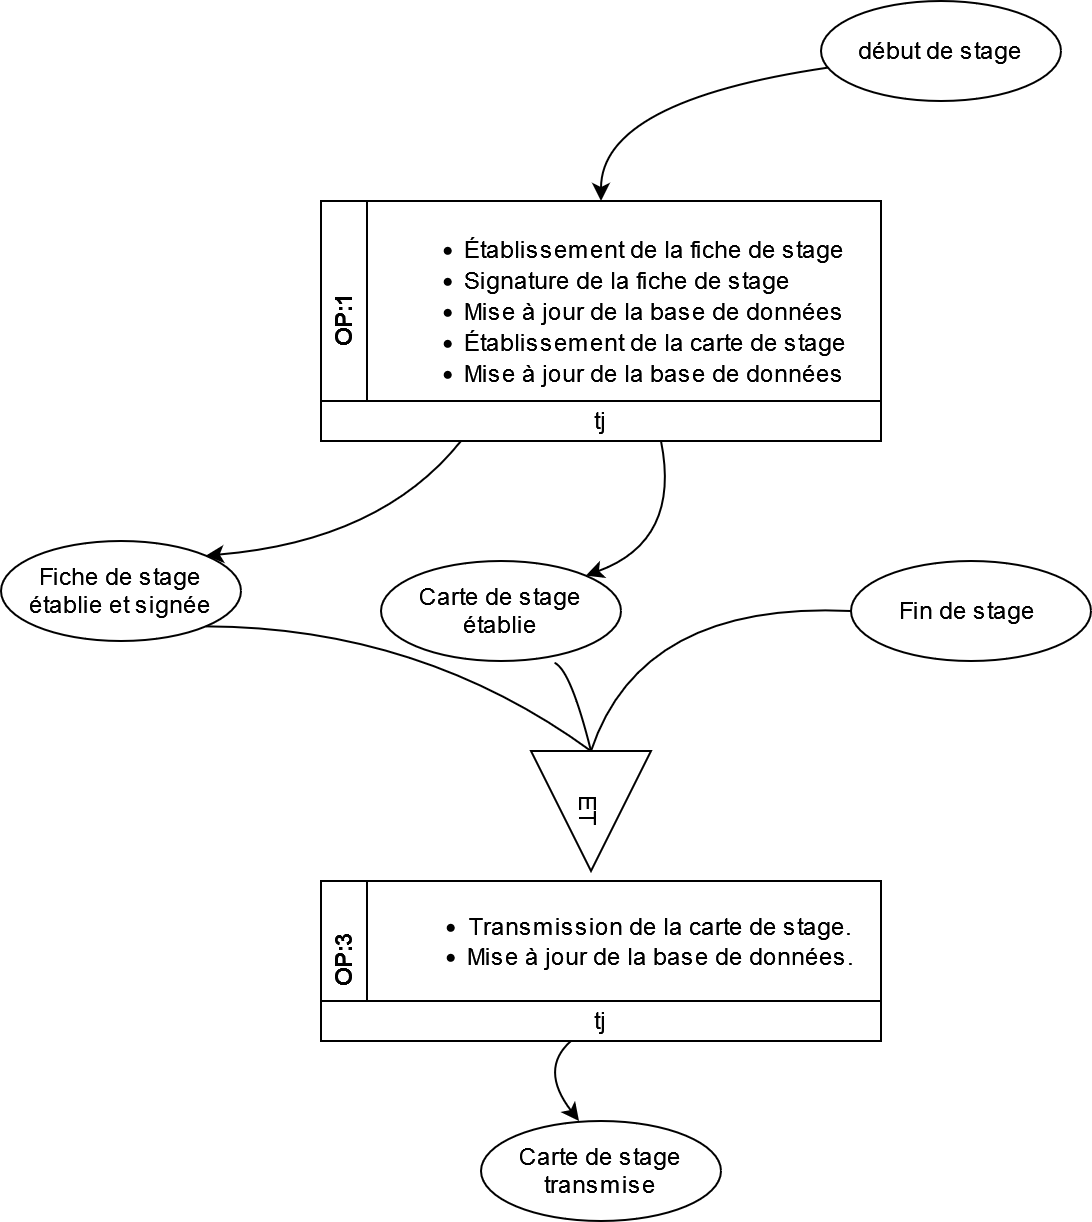
\includegraphics[width=0.7\textwidth]{chapter/Conceptual Study/processus/stage.mct.png}
\subsubsection{process experience}
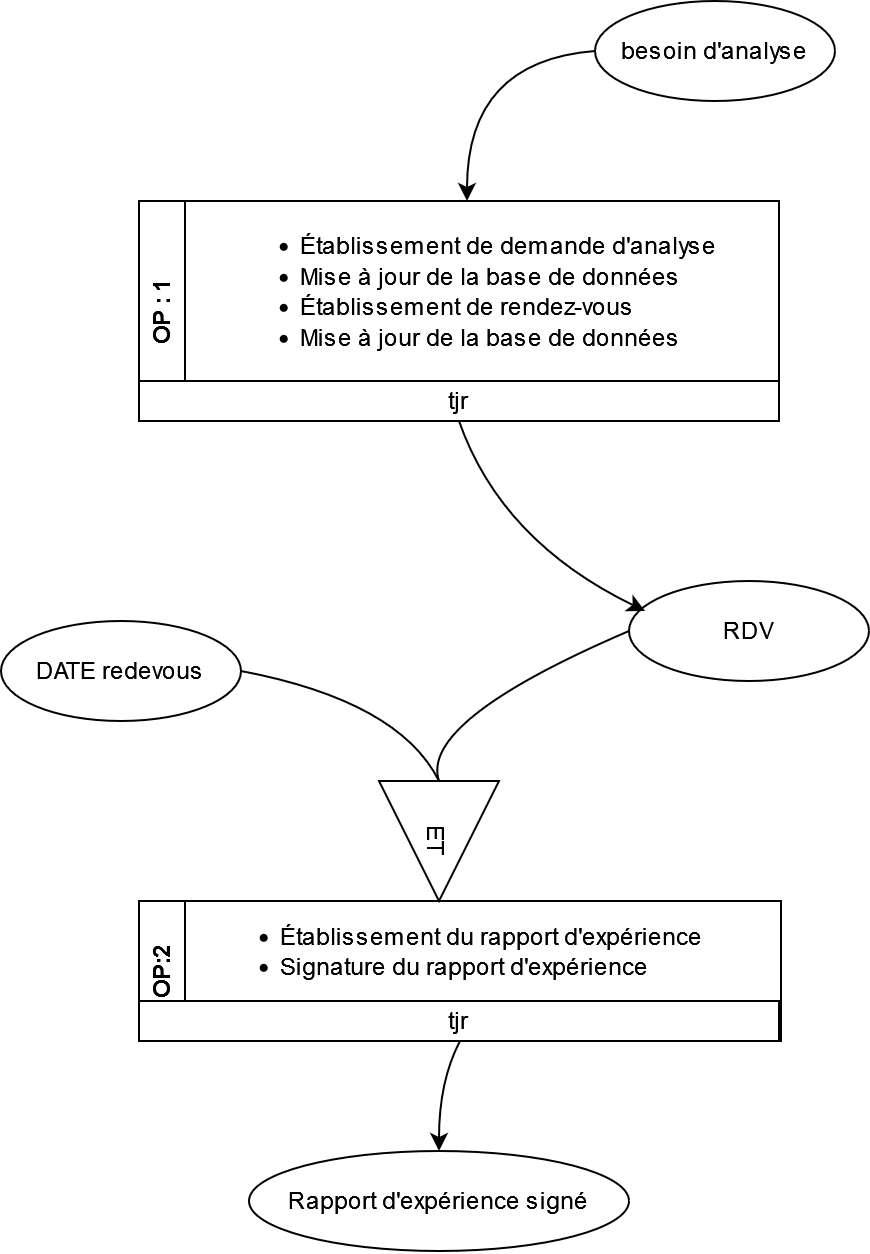
\includegraphics[width=0.7\textwidth]{chapter/Conceptual Study/processus/experience.mct.png}
\subsubsection{process besoin de Produit}
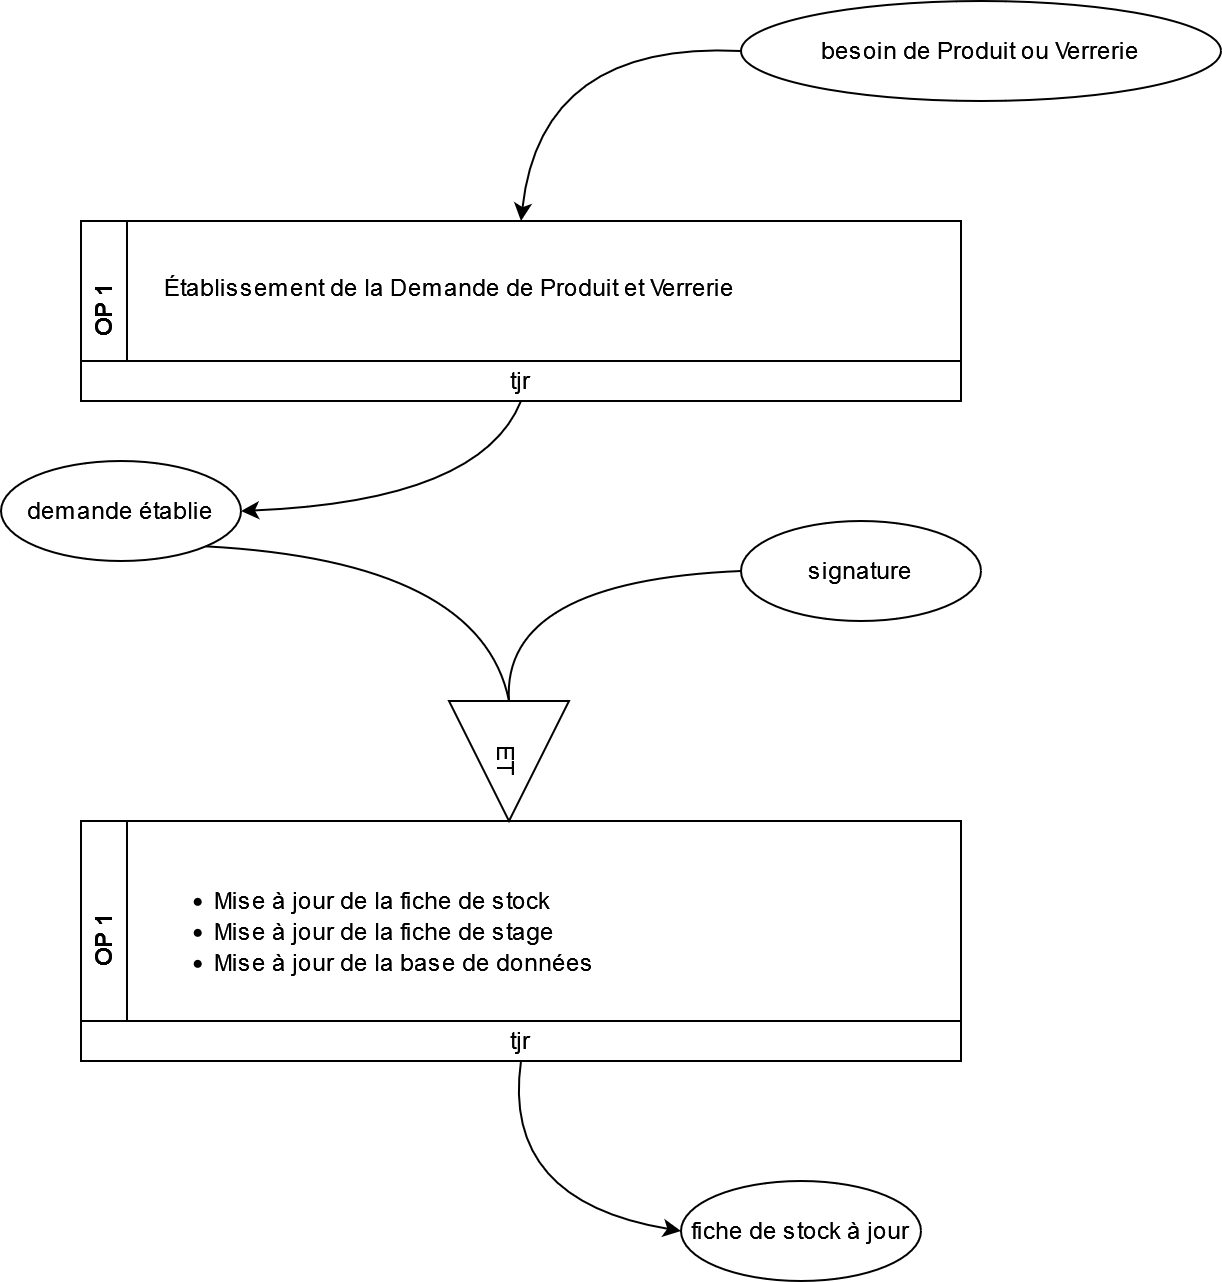
\includegraphics[width=0.7\textwidth]{chapter/Conceptual Study/processus/besoin.mct.png}
\subsubsection{process achat}
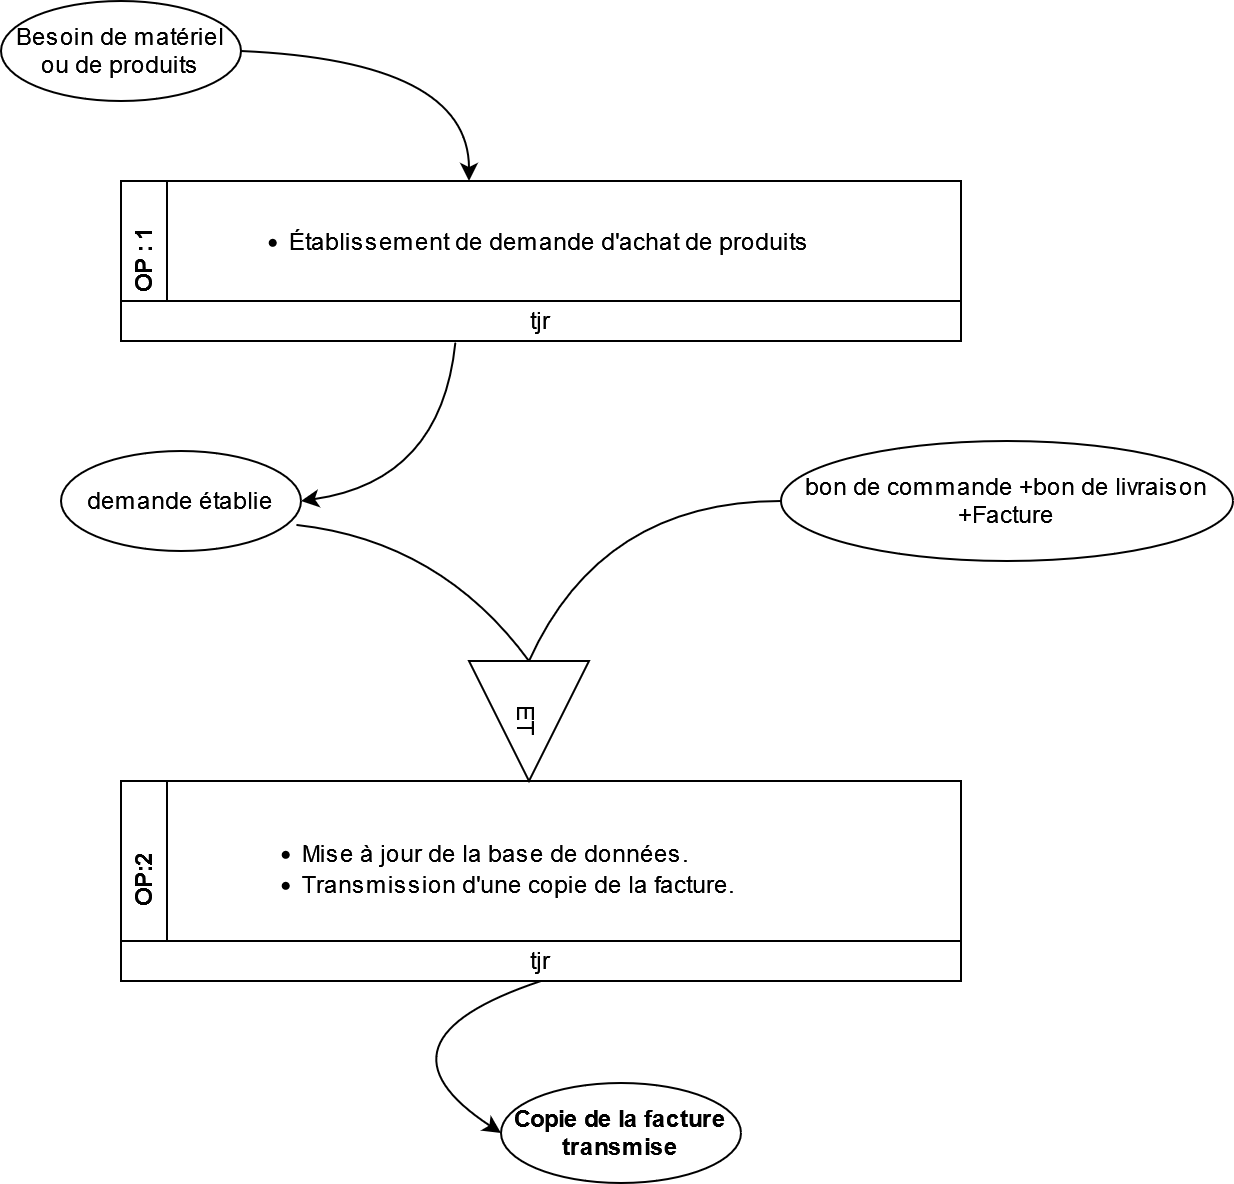
\includegraphics[width=0.7\textwidth]{chapter/Conceptual Study/processus/achat.mct.png}
\subsubsection{process maintenance}
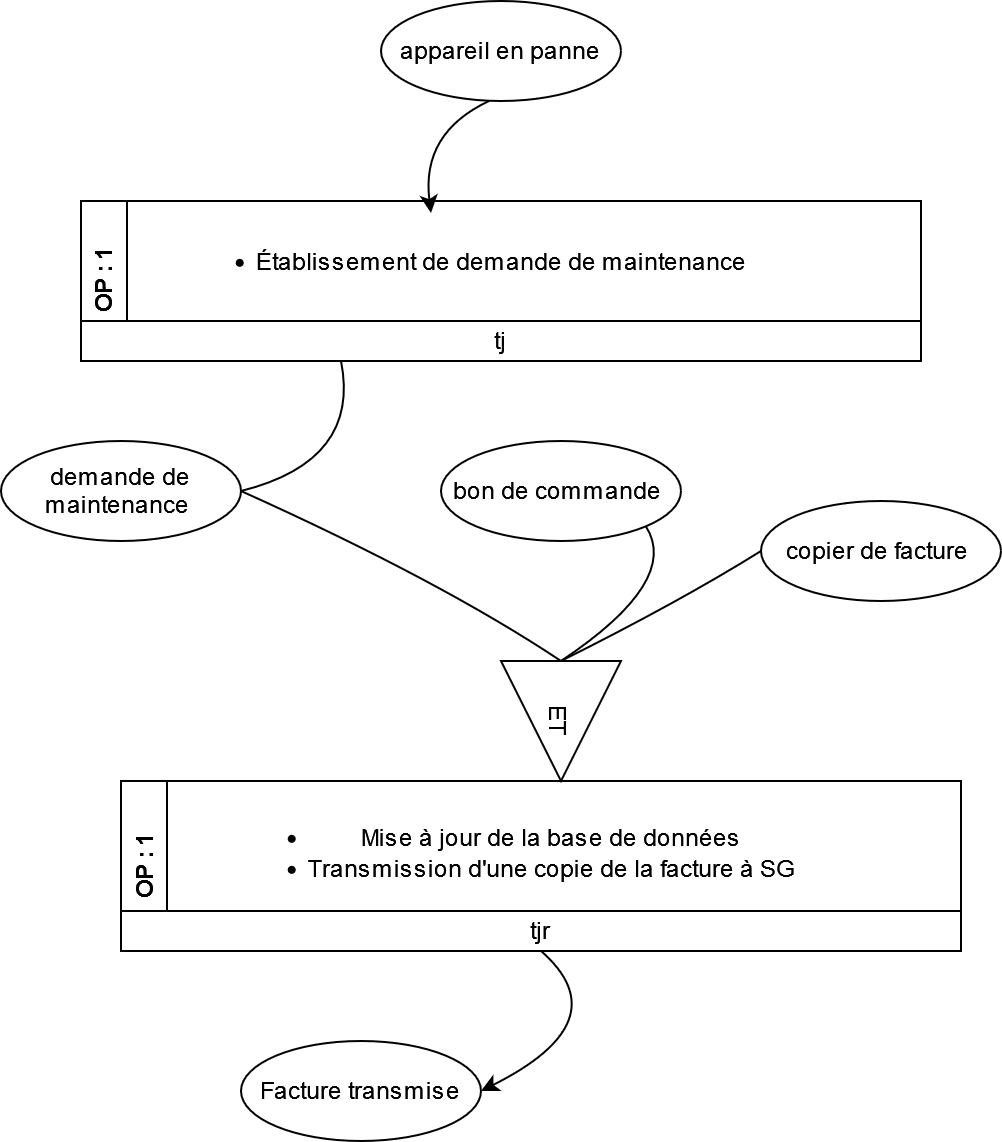
\includegraphics[width=0.7\textwidth]{chapter/Conceptual Study/processus/maintenance.mct.png}
\subsubsection{process inventaire}
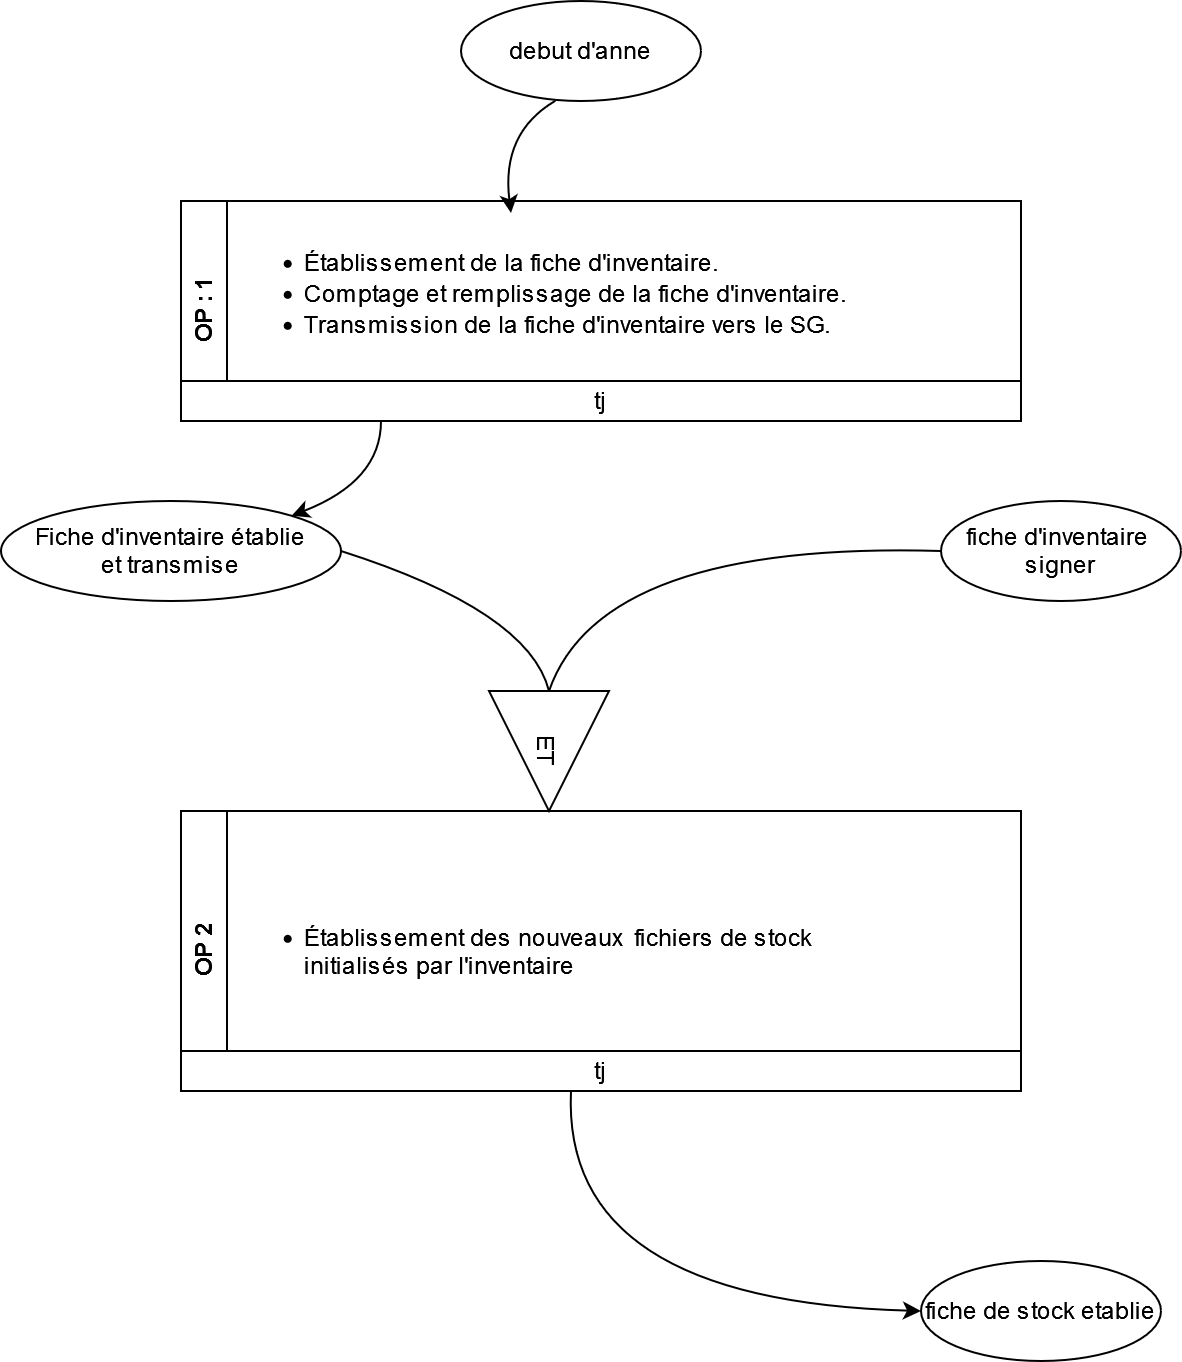
\includegraphics[width=0.7\textwidth]{chapter/Conceptual Study/processus/inventaire.mct.png}

\section{Modèle Organisationnel des traitements}
Le MLT, appelé aussi MOT pour « modèle organisationnel des traitements »,
décrit avec précision l’organisation à mettre en place pour réaliser une ou, le
cas échéant, plusieurs opérations figurant dans le MCT. Il répond aux
questions suivantes : qui ? quoi ? où ? quand ? À un MCT correspondent donc
généralement plusieurs MLT.
Les notions introduites à ce niveau sont : le poste de travail, la phase, la tâche
et la procédure.
Le poste de travail
Le poste de travail décrit la localisation, les responsabilités, et les
ressources nécessaires pour chaque profil d’utilisateur du système.
La phase
La phase est un ensemble d’actions (cf. la notion d’opération pour le
MCT) réalisées sur un même poste de travail.
La phase peut être :
soit manuelle : par exemple, la confection d'un colis ;
soit automatisée et interactive : par exemple, la saisie d’un
formulaire client ;
soit automatisée et planifiée (on parle aussi de batch) : par exemple,
la production et l'envoi quotidiens de tableaux de bord dans les
boites aux lettres électroniques.

La tâche
La tâche est une description détaillée d’une phase automatisée
interactive.
La procédure
La procédure est un regroupement de phases. Elle équivaut sur le plan de
l’organisation aux notions d’opérations et d’actions conceptuelles. La
différence est que l'on considère ici ces dernières comme se déroulant sur
une période de temps homogène.
Des procédures d’origines non conceptuelles peuvent être ajoutées du fait
des choix d’organisation effectués.
\subsection{procedure}
\newpage -\newpage- \newpage -\newpage -\newpage -\newpage 
%\includegraphics[width=1\textwidth]{chapter/Conceptual Study/procedures/analyse.png}